\documentclass[11pt,twoside]{book}

\usepackage[T1]{fontenc}
\usepackage[utf8]{inputenc}
\usepackage{lmodern}
\usepackage[paperwidth=6in,paperheight=9in,top=0.85in,bottom=0.9in,inner=0.9in,outer=0.7in,bindingoffset=0.3in]{geometry}
\usepackage{xcolor}
\usepackage{tikz}
\usetikzlibrary{positioning,calc,shapes.geometric,backgrounds}
\usepackage{lettrine}
\usepackage{microtype}
\usepackage{booktabs}
\usepackage{array}
\usepackage{tcolorbox}
\tcbuselibrary{skins}

\definecolor{inkblack}{HTML}{1B1B1B}
\definecolor{burgundy}{HTML}{6E2036}
\definecolor{softgray}{HTML}{6F6F6F}
\definecolor{parchment}{HTML}{F3EEE3}

\color{inkblack}

\newcommand{\chapterornament}{%
\begin{center}

\begin{tikzpicture}
\draw[burgundy, line width=0.6pt] (-1.3,0) -- (-0.22,0);
\draw[burgundy, line width=0.6pt] (0.22,0) -- (1.3,0);
\node[regular polygon, regular polygon sides=4, draw=burgundy, fill=burgundy, minimum size=6pt, inner sep=0pt] at (0,0) {};
\end{tikzpicture}
\end{center}}

\newcommand{\novelchapter}[2]{%
\clearpage
\thispagestyle{empty}
\vspace*{0.55in}
\begin{center}
{\fontsize{10}{12}\selectfont\color{softgray}\MakeUppercase{Chapter #1}}\\[0.4em]
{\fontsize{25}{29}\selectfont\bfseries\color{inkblack} #2}\\[0.55em]
\chapterornament
\end{center}
\vspace{0.45in}}

\newcommand{\sceneBreak}{%
\par\vspace{1.1em}
\begin{center}\textcolor{burgundy}{$\ast$~~$\ast$~~$\ast$}\end{center}
\vspace{1.1em}}

\begin{document}

% ---------- HALF-TITLE ----------
\thispagestyle{empty}
\pagenumbering{roman}
\null
\vspace*{2.4in}
\begin{center}
{\fontsize{15}{18}\selectfont\itshape\color{softgray} The Meridian Line}
\end{center}
\clearpage

% ---------- TITLE PAGE ----------
\thispagestyle{empty}
\null
\vspace*{1.3in}
\begin{center}
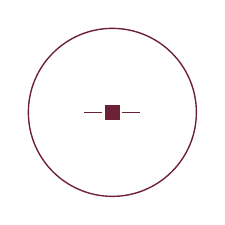
\begin{tikzpicture}
\draw[burgundy, line width=0.5pt] (0,0) circle (0.42in);
\node[regular polygon, regular polygon sides=4, draw=burgundy, fill=burgundy, minimum size=7pt, inner sep=0pt] at (0,0) {};
\draw[burgundy, line width=0.5pt] (-0.14in,0) -- (-0.05in,0);
\draw[burgundy, line width=0.5pt] (0.05in,0) -- (0.14in,0);
\end{tikzpicture}\\[0.5in]
{\fontsize{30}{34}\selectfont\bfseries\color{inkblack} The Meridian\\[0.1em] Line}\\[0.55in]
{\fontsize{13}{15}\selectfont\itshape\color{softgray} a novel}\\[1.4in]
{\fontsize{13}{16}\selectfont\color{inkblack} Elena Kastrinos}
\end{center}
\vfill
\begin{center}
{\fontsize{9}{11}\selectfont\color{softgray}\MakeUppercase{Nimbus Press}}
\end{center}
\vspace{0.35in}
\clearpage

% ---------- COPYRIGHT ----------
\thispagestyle{empty}
\null
\vspace*{2.6in}
\begin{center}
\begin{minipage}{3.6in}
\fontsize{8.5}{11}\selectfont\color{softgray}
\raggedright
Copyright \copyright\ 2026 by Elena Kastrinos

\medskip
All rights reserved. No part of this publication may be reproduced, distributed, or transmitted in any form or by any means, including photocopying, recording, or other electronic or mechanical methods, without the prior written permission of the publisher, except in the case of brief quotations embodied in critical reviews and certain other noncommercial uses permitted by copyright law.

\medskip
This is a work of fiction. Names, characters, places, and incidents either are products of the author's imagination or are used fictitiously. Any resemblance to actual persons, living or dead, events, or locales is entirely coincidental.

\medskip
Published by Nimbus Press

\smallskip
ISBN 978-x-xxxxx-xxx-x (paperback)

\smallskip
First Edition

\smallskip
Printed by Vertex Print Works

\smallskip
Text set in Latin Modern, 11 pt on 14 pt leading, on a 6 \(\times\) 9 in.\ trim.
\end{minipage}
\end{center}
\clearpage

% ---------- DEDICATION ----------
\thispagestyle{empty}
\null
\vspace*{2.7in}
\begin{center}
{\fontsize{12}{16}\selectfont\itshape\color{inkblack}
For everyone who has ever followed\\ a coastline just to see where it leads.}
\end{center}
\clearpage

% ---------- PRODUCTION / TRIM SPECIFICATION ----------
\thispagestyle{empty}
\begin{center}
{\fontsize{11}{13}\selectfont\color{softgray}\MakeUppercase{Production Specification}}\\[0.5em]
\chapterornament
\end{center}
\vspace{0.3in}

\begin{center}
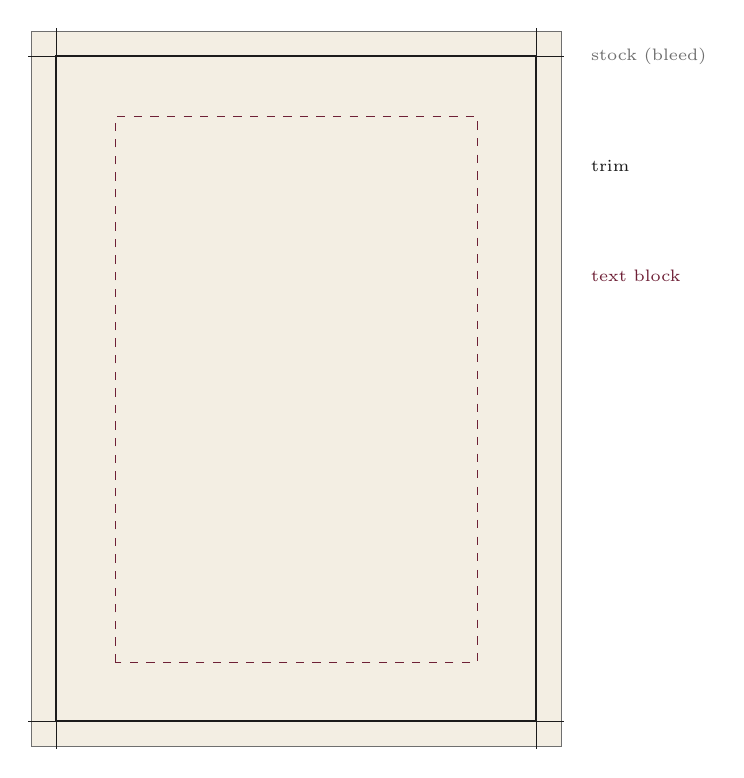
\begin{tikzpicture}[x=1in,y=1in]
  % bleed / stock box
  \fill[parchment] (0,0) rectangle (2.65,3.575);
  \draw[softgray, line width=0.4pt] (0,0) rectangle (2.65,3.575);
  % trim box
  \draw[inkblack, line width=0.7pt] (0.125,0.125) rectangle (2.525,3.45);
  % text block
  \draw[burgundy, line width=0.5pt, dashed] (0.42,0.42) rectangle (2.23,3.15);
  % crop marks
  \foreach \x/\y/\dx/\dy in {0.125/0.125/-1/-1, 2.525/0.125/1/-1, 0.125/3.45/-1/1, 2.525/3.45/1/1}{
    \draw[inkblack, line width=0.4pt] (\x,\y) -- ({\x+\dx*0.14},\y);
    \draw[inkblack, line width=0.4pt] (\x,\y) -- (\x,{\y+\dy*0.14});
  }
  \node[anchor=west, font=\fontsize{6.5}{8}\selectfont\color{softgray}] at (2.75,3.45) {stock (bleed)};
  \node[anchor=west, font=\fontsize{6.5}{8}\selectfont\color{inkblack}] at (2.75,2.9) {trim};
  \node[anchor=west, font=\fontsize{6.5}{8}\selectfont\color{burgundy}] at (2.75,2.35) {text block};
\end{tikzpicture}
\end{center}
\vspace{0.15in}
{\footnotesize\color{softgray}\centering Diagram schematic, not to scale.\par}
\vspace{0.35in}

\begin{center}
\begin{tabular}{@{}ll@{}}
\toprule
\textbf{Trim size} & 6 in \(\times\) 9 in \\
\textbf{Bleed} & 0.125 in on all edges \\
\textbf{Binding offset} & 0.3 in \\
\textbf{Margins (in.\ / out.)} & 0.9 in / 0.7 in \\
\textbf{Margins (top / bot.)} & 0.85 in / 0.9 in \\
\textbf{Type} & Latin Modern, 11/14 pt \\
\bottomrule
\end{tabular}
\end{center}
\clearpage

% ---------- MAIN MATTER ----------
\pagenumbering{arabic}
\pagestyle{plain}

\novelchapter{One}{Landfall}

\lettrine[lines=3,slope=0.4em,findent=0.1em,nindent=0em]{\color{burgundy}T}{he} chart had been wrong for eleven years before anyone thought to check it against the water itself. Marisol Andeen found the discrepancy on a Tuesday, kneeling on the wet rocks below the Cape Isolde light with a plumb line in one hand and her grandfather's brass sextant in the other, and for a long moment she simply watched the tide erase her footprints and said nothing at all.

The coastline, according to the Admiralty survey of 1962, ran due north-northeast from the lighthouse for four hundred meters before curving inland around a shoal that no longer existed. Marisol had sailed past that shoal a hundred times as a child, had watched her father steer wide of it out of habit rather than necessity, and had never once asked why a rock that showed on every chart in the harbormaster's office had not shown itself to her in twenty-two years of looking. Now she knew. The shoal was gone, worn down by decades of current, and the coastline behind it had crept forward to fill the space, patient as only stone and water can be patient.

She measured the new angle three times before she trusted it. Then she opened her field notebook, the one with the salt-stained cover that her mother had given her the week she left the university, and began to draw the coastline as it actually was rather than as it had been recorded. It was slow work. Every inlet had to be walked, every rock face measured against the last known fixed point, every old assumption tested and, more often than not, discarded. By the time the light began to fail she had covered perhaps sixty meters of shoreline, and she felt, for the first time since she had accepted this absurd commission from a dying newspaper's dying cartography desk, that she was doing something that mattered.

\sceneBreak

The letter had arrived on the same morning as her reassignment papers, tucked into the same envelope as though the postal service itself had decided the two things belonged together. It was addressed to a woman named Ines Calder, forwarded from an address in the old fishing quarter that had been condemned for twenty years, and it was written in a hand so careful and so cramped that Marisol had needed her grandfather's magnifying glass to read the first line: \emph{By the time this reaches you, the meridian will have moved again, and I will not have told you why.}

She should have returned it. Instead she read it twice, folded it back along its original creases, and placed it inside the same notebook where she was redrawing the coast — as if the two mysteries, the moving shoreline and the moving meridian, might somehow explain each other if she simply kept them close enough together.

\novelchapter{Two}{The Harbormaster's Ledger}

The harbormaster's office at Cape Isolde had not been renovated since the light itself was electrified, and it showed its age in the particular way that government buildings on forgotten coastlines always did: peeling paint above the waterline, immaculate order below it. Petros Vann kept forty years of tide tables in a locked cabinet behind his desk, and he unlocked it for Marisol only after she had explained, twice, that she was not there to close anything down.

\begin{quote}
\itshape ``Nobody surveys this coast because nobody profits from this coast,'' he told her, sliding a ledger across the desk with the reluctance of a man handing over something he had never expected to need again. ``You'll want the volume from sixty-one. That's the year the numbers stop matching the rocks.''
\end{quote}

She found the entry before she found the reason for it: a single line, dated the fourteenth of March, noting a triangulation reading that placed the Cape Isolde meridian marker four arc-seconds west of where it had stood the previous survey. Four arc-seconds was nothing to a sailor and everything to a cartographer. Four arc-seconds, walked forward year after year, was exactly enough to explain a shoal that had wandered out of a hundred honest charts and into the sea.

What it did not explain was why someone had gone to the trouble of writing to a woman who no longer lived at the only address anyone had for her, in a hand shaking with an urgency that had nothing to do with rocks. Marisol copied the triangulation figures into her own notebook, thanked Petros Vann for his trouble, and walked back out into a wind that smelled, unmistakably, of a coastline about to change its mind again.

\sceneBreak

That night she read the letter a third time, and on the third reading she noticed what she had missed twice before: a postscript, added in a different ink, giving not an address but a set of coordinates. She did not yet know what waited at the far end of them. She knew only that the meridian had moved once before without anyone troubling to write it down, and that this time, whatever else happened, someone intended it to be witnessed.

\clearpage
\thispagestyle{empty}
\null
\vspace*{2.5in}
\begin{center}
{\fontsize{10}{12}\selectfont\color{softgray}\MakeUppercase{End of Sample}}
\end{center}
\clearpage

% ---------- ABOUT THE AUTHOR ----------
\thispagestyle{empty}
\begin{center}
{\fontsize{11}{13}\selectfont\color{softgray}\MakeUppercase{About the Author}}\\[0.5em]
\chapterornament
\end{center}
\vspace{0.3in}
{\fontsize{10.5}{15}\selectfont
Elena Kastrinos grew up on a working harbor and spent a decade surveying coastlines before she began writing fiction about the people who draw them. \emph{The Meridian Line} is her first novel. She lives, as she always has, within sight of the water.\par}

\vspace{0.6in}
\begin{center}
{\fontsize{9}{11}\selectfont\color{softgray}\MakeUppercase{Colophon}}\\[0.5em]
\chapterornament
\end{center}
\vspace{0.2in}
{\fontsize{8.5}{11}\selectfont\color{softgray}\raggedright\noindent
This book was typeset in Latin Modern, a scalable descendant of Computer Modern, at 11 points on 14 points of leading, within a 6 \(\times\) 9 in.\ trim with a 0.125 in.\ bleed and a 0.3 in.\ binding offset. Chapter openings use a hand-set ornament in a single accent color; scene breaks are marked with a centered triad rather than a rule, to keep the page quiet. Composed with \LaTeX\ using a dedicated novel-layout page geometry and custom chapter styling.\par}

\end{document}
